% Beijing National Day School General LaTex style 
% This is unofficial so you can modified it by yourself
% See https://bndsecon.com/ for more information in BNDS
% To be honest, this is my school project so it may be a little bit haste

% ------------------------------------------------------------------------------------------
% Features 1: You can modified the font size at here. I provide three font sizes: 10pt 11pt 12pt
% Remember! You need to comment the rest of the two options codes 
% \documentclass[10pt]{report}
% \documentclass[11pt]{report}

\documentclass[12pt, a4paper, oneside]{report}
% ------------------------------------------------------------------------------------------


\usepackage{fancyhdr}
\usepackage{graphicx}
\usepackage{tikz}
\usepackage{qrcode} % QR code generator 
\usepackage{gensymb}  % \degree
\usepackage{pgfornament}
\usepackage{eso-pic}
\usepackage{siunitx}
\usepackage{tikzrput}
\usepackage{tabularx}
\usepackage{fontspec}
\usepackage{longtable}
\usepackage{lipsum}
\usepackage{setspace}
\usepackage{hyperref}
\usepackage{amsmath, amsthm, amssymb, appendix, bm, mathrsfs,extarrows}
\usepackage{abstract}
\usepackage{esint}
\usepackage[autostyle, english = american]{csquotes}  % quote orientation
\DeclareGraphicsExtensions{.png,.pdf}
% ------------------------------------------------------------------------------------------
% Features 2: You can modified the page margins at here

\usepackage[top=1in,bottom=1in,left=1in,right=1in,xetex]{geometry}
% ------------------------------------------------------------------------------------------

% ------------------------------------------------------------------------------------------
% Features 3: You can modified the line spread at here. 
%             1 is default 
%             1.3 is pretty good
% \linespread{0.8}
% \linespread{1}
\linespread{1.3}
% \linespread{1.5}
% \linespread{2} 
% ------------------------------------------------------------------------------------------




% ------------------------------------------------------------------------------------------
% Features 4: You can modified the font at here, I give you a very elegant font 

% \setmainfont{texgyrepagella-regular.otf}[
% BoldFont = texgyrepagella-bold.otf ,
% ItalicFont = texgyrepagella-italic.otf ,
% BoldItalicFont = texgyrepagella-bolditalic.otf ]

% \setsansfont{texgyrepagella-regular.otf}[
% BoldFont = texgyrepagella-bold.otf ,
% ItalicFont = texgyrepagella-italic.otf ,
% BoldItalicFont = texgyrepagella-bolditalic.otf ]

% \setmonofont{texgyrepagella-regular.otf}[
% BoldFont = texgyrepagella-bold.otf ,
% ItalicFont = texgyrepagella-italic.otf ,
% BoldItalicFont = texgyrepagella-bolditalic.otf ]


% ------------------------------------------------------------------------------------------




% ------------------------------------------------------------------------------------------
% Features 5: I have carefully prepared the page decoration for you. You can check out more decorations on this official website  
% https://ctan.org/pkg/pgfornament


% \usetikzlibrary{positioning, arrows.meta, chains, scopes, calc}
% \newcommand\AtPageUpperRight[1]{\AtPageUpperLeft{%
% \put(\LenToUnit{\paperwidth},\LenToUnit{0\paperheight}){#1}%
%  }}%
% \newcommand\AtPageLowerRight[1]{\AtPageLowerLeft{%
% \put(\LenToUnit{\paperwidth},\LenToUnit{0\paperheight}){#1}%
% }}%
% \AddToShipoutPictureBG{%
%   \AtPageUpperLeft{\put(0,-25){\pgfornament[width=1.75cm]{39}}}
%   \AtPageUpperRight{\put(-50,-25){\pgfornament[width=1.75cm,symmetry=v]{39}}}
%   \AtPageLowerLeft{\put(0,25){\pgfornament[width=1.75cm,symmetry=h]{39}}}
%   \AtPageLowerRight{\put(-50,25){\pgfornament[width=1.75cm,symmetry=c]{39}}}
% }
%
% ------------------------------------------------------------------------------------------

\MakeOuterQuote{"}



% ------------------------------------------------------------------------------------------
% Features 6: I provide you a fancy head at here. You can change the name or the logo here


% \fancyhf{}
% \fancyhead[L]{
% 	\begin{minipage}[c]{0.06\textwidth}
% 		
\includegraphics[height=7.5mm]{pic\BNDS_Logo_Horizon.png}
% 	\end{minipage}
% 	\begin{minipage}[c]{0.4\textwidth}
% 	You can write anything here.
% 	\end{minipage}}
% \fancyhead[R]{Your Title / Author name}




% ------------------------------------------------------------------------------------------


% ------------------------------------------------------------------------------------------
% Features 6: I provide you a fancy foot at here. You can change the name or the logo here


% \fancyfoot[L]{
% 	\begin{minipage}[c]{0.06\textwidth}
% 		
\includegraphics[height=7.5mm]{pic\BNDS_Logo_Small.png}
% 	\end{minipage}}
% \fancyfoot[R]{
% 	\begin{minipage}[c]{0.06\textwidth}
% 		
\includegraphics[height=7.5mm]{pic\BNDS_Logo_Small.png}
% 	\end{minipage}}
% \fancyfoot[C]{ \thepage }

% \pagestyle{fancy}

% ------------------------------------------------------------------------------------------




\title{Enter Your Title Here}
\author{Your Name \pgfornament[width=0.7cm]{94}}
\date{\today}


\renewcommand{\abstractname}{\Large\textbf{Abstract}}
\renewcommand\thesection{\arabic {section}}
\begin{document}

\maketitle

% ------------------------------------------------------------------------------------------
% Features 6: This is your abstract


\setcounter{page}{1}
\maketitle
\thispagestyle{empty}

\begin{abstract}
    Abstract is one of the most important part for your paper. Make it clear and logical. 
    \par\textbf{Key Word:List your important terms and nones here. }
\end{abstract}

\newpage

% ------------------------------------------------------------------------------------------


% ------------------------------------------------------------------------------------------
% Features 6: This is your abstract


\pagenumbering{Roman}
\setcounter{page}{1}
\tableofcontents
\newpage

\setcounter{page}{1}
\pagenumbering{arabic}


% ------------------------------------------------------------------------------------------


\section{Introduction}


\section{Model}

\lipsum[1-3]

\begin{figure}
    \centering
    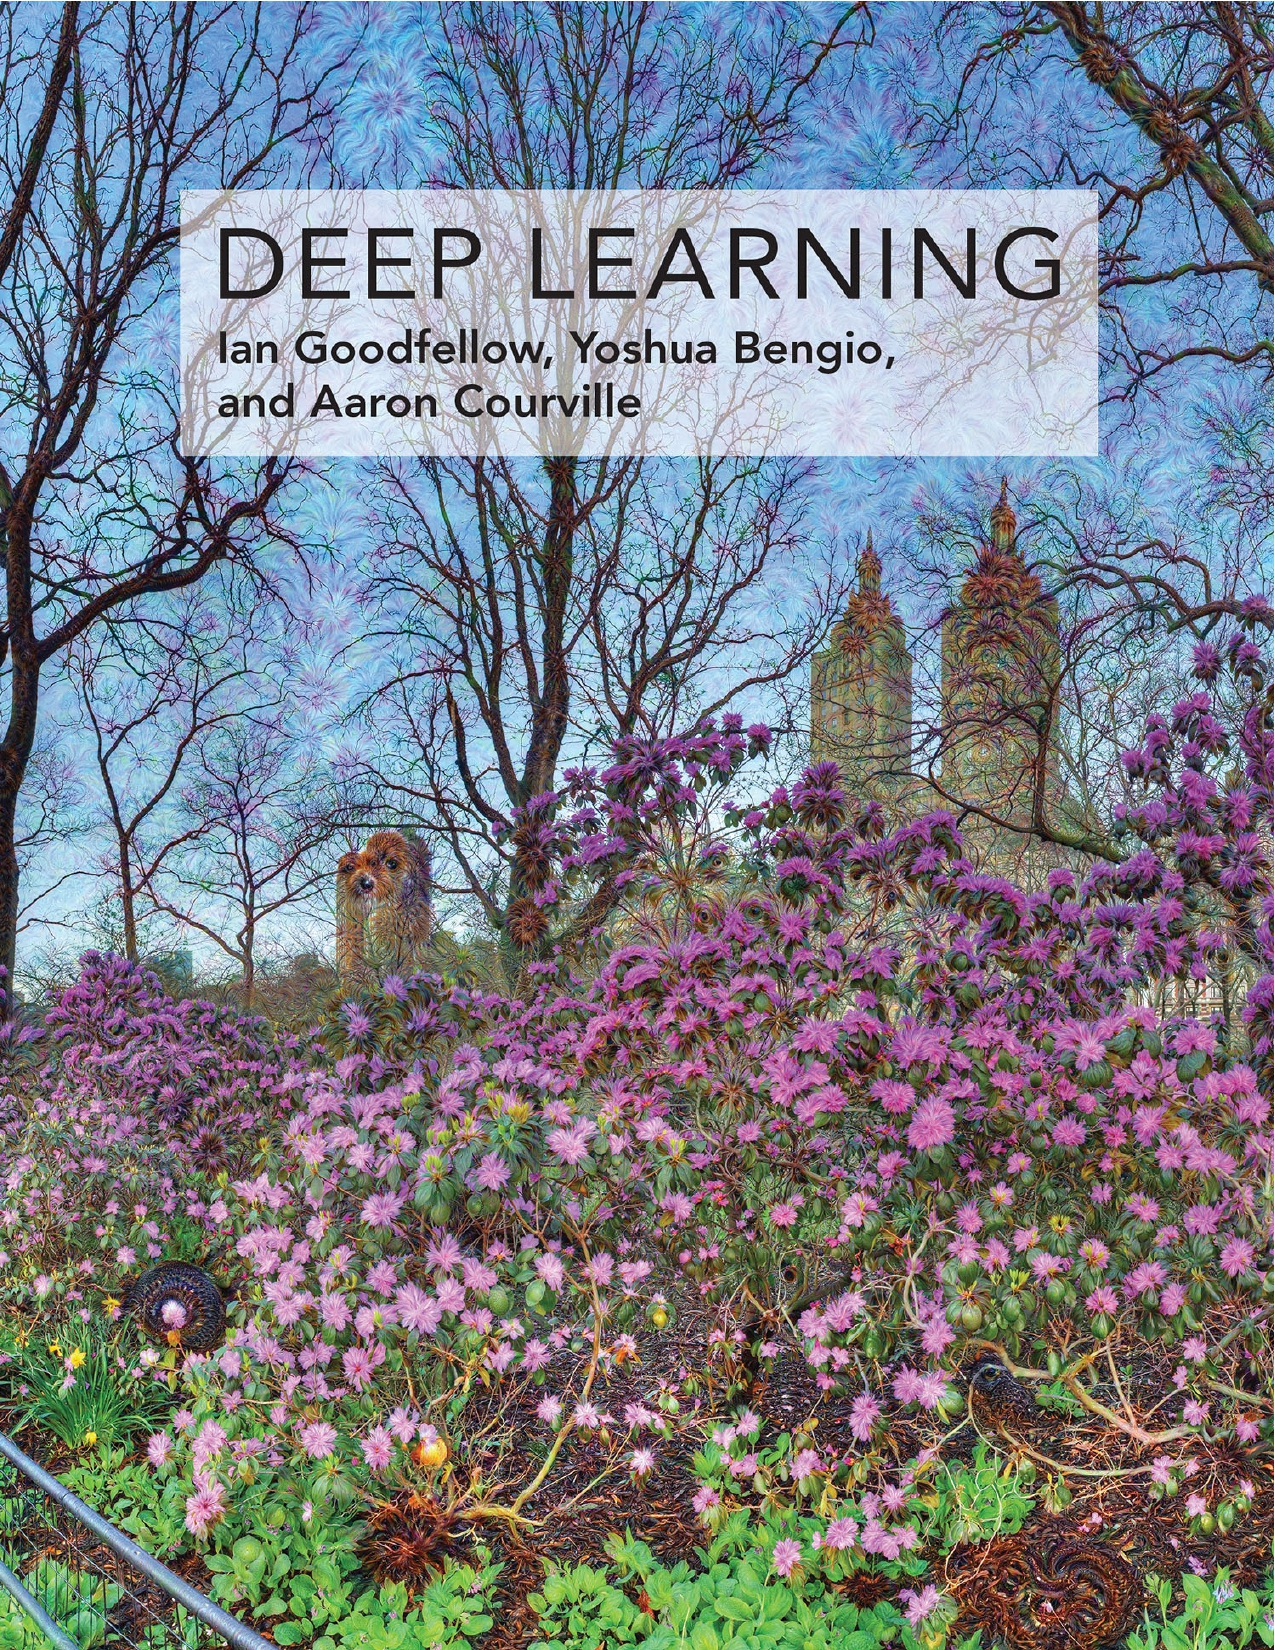
\includegraphics[width=6cm]{pic/DeepLearning.jpg}
\end{figure}

\subsection{Short - Term model}
\lipsum[4-6]
\begin{equation}
    \nabla f\left( \boldsymbol{x} \right) =\mathbf{grad}f\left( \boldsymbol{x} \right) \xlongequal{\mathrm{def}}\left[ \begin{array}{c}
        \frac{\partial f\left( \boldsymbol{x} \right)}{\partial x_1}\\
        \frac{\partial f\left( \boldsymbol{x} \right)}{\partial x_2}\\
        \vdots\\
        \frac{\partial f\left( \boldsymbol{x} \right)}{\partial x_n}\\
    \end{array} \right] 
\end{equation}


\subsection{Long - Term model}
\lipsum[7-9]
\begin{equation}
    \iint_{\varSigma}{\left| \begin{matrix}
        \mathrm{d}y\mathrm{d}z&		\mathrm{d}z\mathrm{d}x&		\mathrm{d}x\mathrm{d}y\\
        \frac{\partial}{\partial x}&		\frac{\partial}{\partial y}&		\frac{\partial}{\partial z}\\
        P&		Q&		R\\
    \end{matrix} \right|}=\oint_{\varGamma}{P\mathrm{d}x+Q\mathrm{d}y+R\mathrm{d}z}
\end{equation}


% ------------------------------------------------------------------------------------------
% Features 6: I have carefully prepared the page decoration for you. You can check out more decorations on this official website  


% uncomment this section for a Appendix insertion
% \appendix
% \chapter{Appendix}

% ------------------------------------------------------------------------------------------







% \bibliographystyle{unsrt}


% ------------------------------------------------------------------------------------------
% Features 7: You can easily manage your reference here


% \bibliography{bibEG}

% ------------------------------------------------------------------------------------------


\newpage

\begin{thebibliography}{99}
    \bibitem{a}reference
    \bibitem{b}reference 
\end{thebibliography}

\newpage

\begin{appendices}
    \renewcommand{\thesection}{\Alph{section}}
    \section{Appendix Title}
        Write your appendix here
\end{appendices}
\end{document}
